% Options for packages loaded elsewhere
\PassOptionsToPackage{unicode}{hyperref}
\PassOptionsToPackage{hyphens}{url}
\PassOptionsToPackage{dvipsnames,svgnames,x11names}{xcolor}
\PassOptionsToPackage{space}{xeCJK}
\documentclass[
  10pt,
]{article}
\usepackage{xcolor}
\usepackage[margin=0.70in]{geometry}
\usepackage{amsmath,amssymb}
\setcounter{secnumdepth}{-\maxdimen} % remove section numbering
\usepackage{iftex}
\ifPDFTeX
  \usepackage[T1]{fontenc}
  \usepackage[utf8]{inputenc}
  \usepackage{textcomp} % provide euro and other symbols
\else % if luatex or xetex
  \usepackage{unicode-math} % this also loads fontspec
  \defaultfontfeatures{Scale=MatchLowercase}
  \defaultfontfeatures[\rmfamily]{Ligatures=TeX,Scale=1}
\fi
\usepackage{lmodern}
\ifPDFTeX\else
  % xetex/luatex font selection
  \setmainfont[]{Cambria}
  \setmonofont[]{Consolas}
  \ifXeTeX
    \usepackage{xeCJK}
    \setCJKmainfont[]{Microsoft YaHei}
  \fi
  \ifLuaTeX
    \usepackage[]{luatexja-fontspec}
    \setmainjfont[]{Microsoft YaHei}
  \fi
\fi
% Use upquote if available, for straight quotes in verbatim environments
\IfFileExists{upquote.sty}{\usepackage{upquote}}{}
\IfFileExists{microtype.sty}{% use microtype if available
  \usepackage[]{microtype}
  \UseMicrotypeSet[protrusion]{basicmath} % disable protrusion for tt fonts
}{}
\makeatletter
\@ifundefined{KOMAClassName}{% if non-KOMA class
  \IfFileExists{parskip.sty}{%
    \usepackage{parskip}
  }{% else
    \setlength{\parindent}{0pt}
    \setlength{\parskip}{6pt plus 2pt minus 1pt}}
}{% if KOMA class
  \KOMAoptions{parskip=half}}
\makeatother
\usepackage{longtable,booktabs,array}
\newcounter{none} % for unnumbered tables
\usepackage{calc} % for calculating minipage widths
% Correct order of tables after \paragraph or \subparagraph
\usepackage{etoolbox}
\makeatletter
\patchcmd\longtable{\par}{\if@noskipsec\mbox{}\fi\par}{}{}
\makeatother
% Allow footnotes in longtable head/foot
\IfFileExists{footnotehyper.sty}{\usepackage{footnotehyper}}{\usepackage{footnote}}
\makesavenoteenv{longtable}
\usepackage{graphicx}
\makeatletter
\newsavebox\pandoc@box
\newcommand*\pandocbounded[1]{% scales image to fit in text height/width
  \sbox\pandoc@box{#1}%
  \Gscale@div\@tempa{\textheight}{\dimexpr\ht\pandoc@box+\dp\pandoc@box\relax}%
  \Gscale@div\@tempb{\linewidth}{\wd\pandoc@box}%
  \ifdim\@tempb\p@<\@tempa\p@\let\@tempa\@tempb\fi% select the smaller of both
  \ifdim\@tempa\p@<\p@\scalebox{\@tempa}{\usebox\pandoc@box}%
  \else\usebox{\pandoc@box}%
  \fi%
}
% Set default figure placement to htbp
\def\fps@figure{htbp}
\makeatother
\setlength{\emergencystretch}{3em} % prevent overfull lines
\providecommand{\tightlist}{%
  \setlength{\itemsep}{0pt}\setlength{\parskip}{0pt}}
\usepackage{bookmark}
\IfFileExists{xurl.sty}{\usepackage{xurl}}{} % add URL line breaks if available
\urlstyle{same}
\hypersetup{
  colorlinks=true,
  linkcolor={Maroon},
  filecolor={Maroon},
  citecolor={Blue},
  urlcolor={Blue},
  pdfcreator={LaTeX via pandoc}}

\author{}
\date{}

\setlength{\textfloatsep}{10pt plus 2pt minus 2pt}
\renewcommand{\figurename}{图}
\begin{document}

\section{Eye Sentinel
漏诊复核与同眼照片分析}\label{eye-sentinel-ux6f0fux8bcaux590dux6838ux4e0eux540cux773cux7167ux7247ux5206ux6790}

2026 年 11 月 18 日 · \href{review-failures.en.md}{English} ·
\href{review-failures.zh.pdf}{PDF}

\textbf{用第二个模型给判阴照片重新排序后，进入复核的漏诊从 16 张增到 24
张。} 在公开青光眼筛查数据集 AIROGS 的 773 张开发照片上，各规则均复核 78
张。EfficientNet-B0 负责原判，ResNet-50
帮助确定哪些判阴照片优先复核。阳性表示参照标签要求转诊，阴性表示无需转诊。漏诊是应转诊却被判阴的照片，误报是无需转诊却被判阳的照片。

按不确定性选图时，模型分数越接近转诊阈值，复核优先级越高。质量灰区在此基础上优先考虑质量分较低的照片。质量分用
0 到 1
表示，越高表示模型估计的图像质量越好。双模型规则沿用质量灰区的判阳名单和判阴复核名额，只调整判阴照片的顺序。

{\def\LTcaptype{none} % do not increment counter
\begin{longtable}[]{@{}llrrr@{}}
\toprule\noalign{}
人群情景 & 复核规则 & 全部错误进复核 & 漏诊进复核 & 每千张仍漏诊 \\
\midrule\noalign{}
\endhead
\bottomrule\noalign{}
\endlastfoot
原开发比例 & 不确定性 & 32.8\% & 30.0\% & 45.3 \\
& 质量灰区 & 32.8\% & 32.0\% & 44.0 \\
& 加入第二模型，重排判阴 & 44.8\% & 48.0\% & 33.6 \\
3.2\% 阳性 & 不确定性 & 57.5\% & 44.0\% & 2.4 \\
& 质量灰区 & 63.2\% & 48.0\% & 2.2 \\
& 加入第二模型，重排判阴 & 65.2\% & 70.0\% & 1.3 \\
\end{longtable}
}

开发集中 380/773 张为转诊阳性。3.2\% 来自 AIROGS
公开训练集，此情景只改变阳性与阴性的比重，按每千张复核 100
张估算。表中的覆盖率以复核前相应类型的错误数为分母，剩余漏诊以全部照片为分母。相对质量灰区，双模型规则多送
8 张漏诊进复核，95\% 区间为 {[}1, 12{]}。在 3.2\% 情景中每千张多送 0.93
张，区间为 {[}0.09,
1.60{]}。区间来自将同一患者或有关联的照片一起抽样后，成对比较两条规则。
\href{https://arxiv.org/html/2302.01738}{AIROGS 原论文}

\begin{figure}
\centering
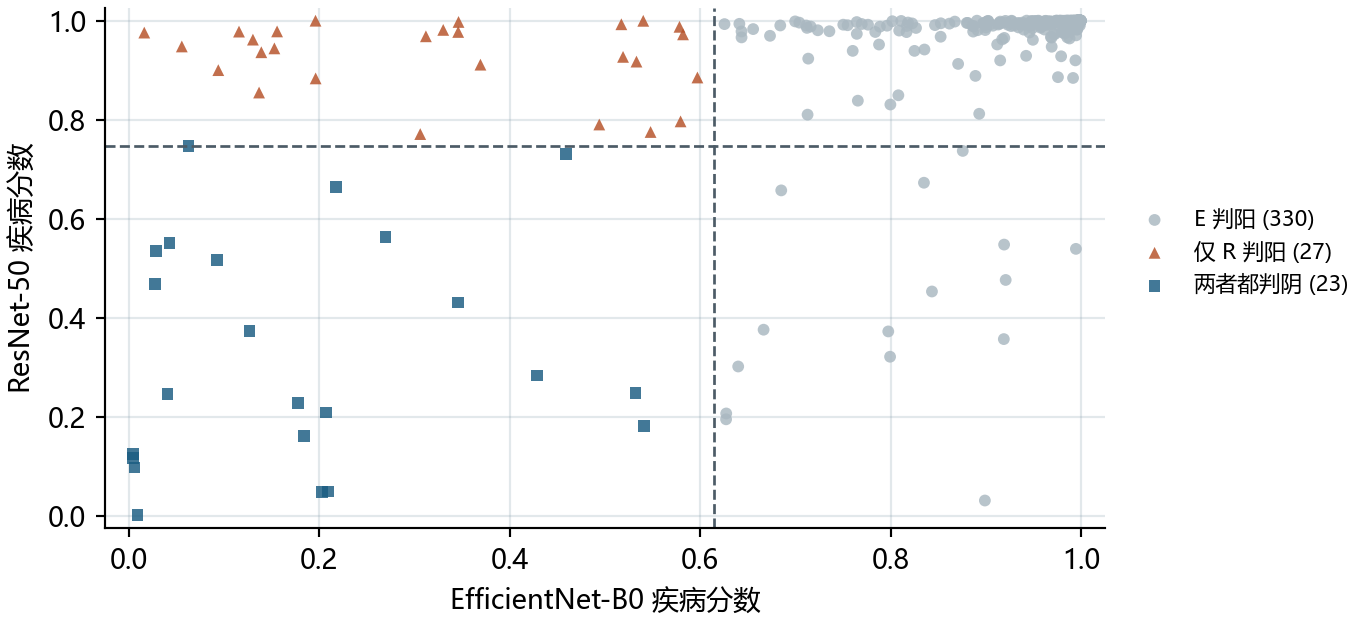
\includegraphics[width=0.88\linewidth,height=\textheight,keepaspectratio,alt={每点代表一张转诊阳性照片。E 指 EfficientNet-B0，R 指 ResNet-50。两条虚线是各自的转诊阈值，超过阈值判阳。}]{review-model-disagreement.zh.png}
\caption{每点代表一张转诊阳性照片。E 指 EfficientNet-B0，R 指
ResNet-50。两条虚线是各自的转诊阈值，超过阈值判阳。}
\end{figure}

EfficientNet-B0 原判漏掉 50 张，ResNet-50 将其中 27
张判阳。质量灰区名单外的 34 个漏诊中，ResNet-50 判阳 15 张，其余 19
张两个模型都判阴。两者都使用第 2,400 次参数更新时保存的模型。组合分数用
767 张模型验证照片拟合，在另外的 773 张开发照片上评估。
\href{backbone-comparison.zh.md}{同协议训练记录}

\newpage

\subsection{照片变糊时，分数怎样动}\label{ux7167ux7247ux53d8ux7ccaux65f6ux5206ux6570ux600eux6837ux52a8}

在同一批 773
张图上模拟轻、强两档失焦，并沿用原来的转诊阈值。原图、轻失焦和强失焦分别漏掉
\textbf{50/380、109/380 和 230/380} 张阳性。强失焦后，348/380
张阳性分数下降，32/380 张上升。185 张从判阳变成漏诊，5
张反向跨过阈值。同一档强失焦下，340/393
张阴性的分数上升，两类因此更难区分。

\begin{figure}
\centering
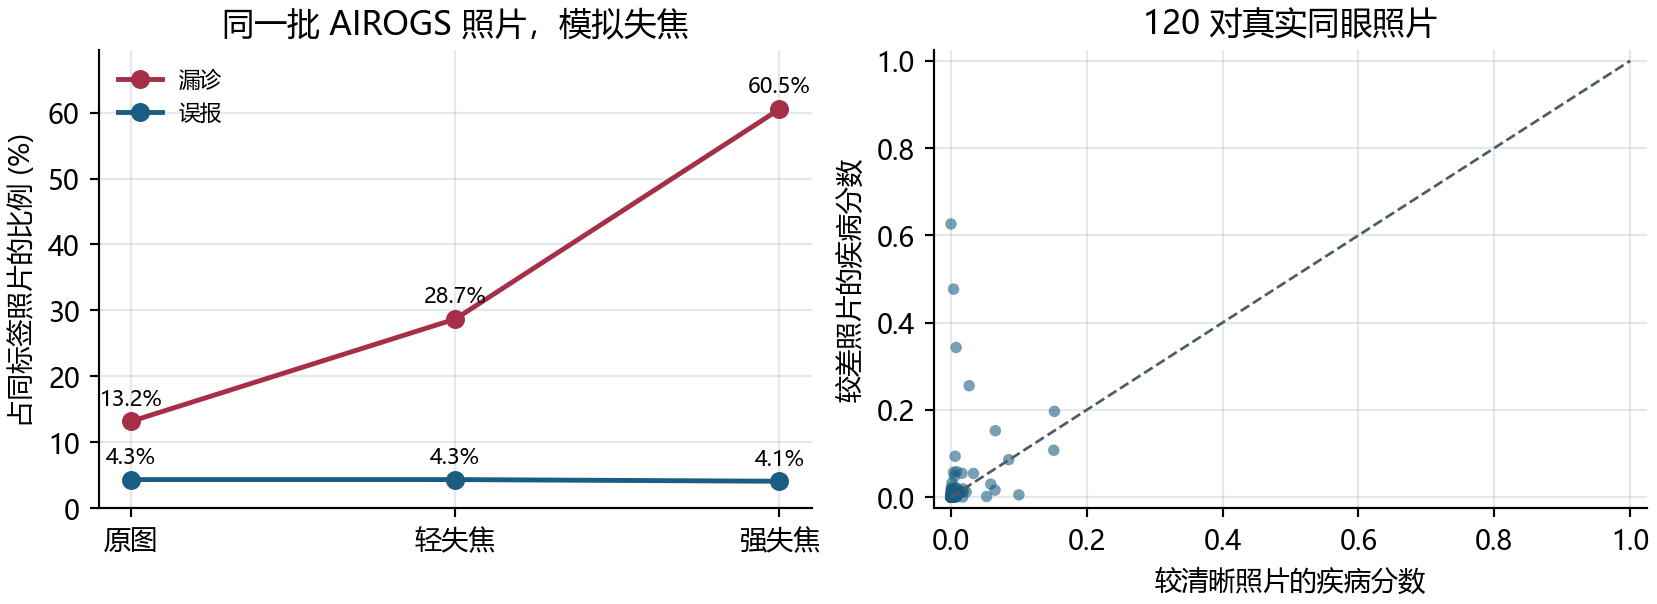
\includegraphics[width=0.98\linewidth,height=\textheight,keepaspectratio,alt={左图在有标签的 AIROGS 图上模拟失焦。右图用 Real Fundus 的真实同眼照片比较较清晰与较差照片的疾病分数，虚线表示两张分数相等。}]{review-paired-focus.zh.png}
\caption{左图在有标签的 AIROGS 图上模拟失焦。右图用 Real Fundus
的真实同眼照片比较较清晰与较差照片的疾病分数，虚线表示两张分数相等。}
\end{figure}

在 \textbf{120 对 Real Fundus 真实同眼照片}中，较差照片的疾病分数有
\textbf{45 对下降、75 对上升}。只有 1
对跨过阈值，较差照片由判阴变为判阳。图像质量变化包含失焦、光照和取景差异。发布数据缺少对应的青光眼参考标签，所以这些数值回答的是模型对同眼不同照片有多敏感。
\href{https://arxiv.org/abs/2201.00466}{Real Fundus 数据论文}

逐图检查发现一张转诊阳性照片的血管轮廓清楚，质量分为
0.89。两个模型给出的转诊分数分别为 0.35 和
0.43，均低于各自阈值，重排后仍在复核名单外。后续可请阅片者在看不到模型原判的情况下检查视盘及其中央凹陷，也就是视杯。

\subsection{对下一轮验证的决定}\label{ux5bf9ux4e0bux4e00ux8f6eux9a8cux8bc1ux7684ux51b3ux5b9a}

以现有质量灰区为对照，优先收集带独立参考检查结果的首拍和重拍，记录视盘和视杯能否判读。在目标站点连续纳入患者，按每百人复核十人，统计剩余漏诊及专家净纠正的错误，也就是改对的数量减去新判错的数量。本轮用一组训练得到的模型在开发照片上评估选图，实际阅片和重拍收益仍待测。预留独立测试集仍封存。

\href{review-failures-results.json}{汇总数据与输入哈希} ·
\href{../../../tools/analyze_review_failures_20261118.py}{分析脚本} ·
\href{../../../tools/plot_review_failures_20261118.py}{绘图脚本}

\end{document}
